\documentclass[10 pt, a4paper]{article}

\usepackage{graphicx}
\usepackage{caption}
\usepackage{anysize}
\usepackage{changepage}
\usepackage{amsfonts}
\usepackage{float}
\usepackage{todonotes}
\usepackage{amsmath}
\usepackage[toc,page]{appendix}
\usepackage{subcaption}
\usepackage{hyperref}

\marginsize{2 cm}{2 cm}{1 cm}{2 cm}

\captionsetup[figure]{labelfont=bf,textfont=it,width=0.88\textwidth}
\captionsetup[table]{labelfont=bf,textfont=it,width=0.88\textwidth}

\setlength{\parindent}{0 cm}

\begin{document}

\begin{center}
\huge The Effect of Varying the Numer of Hidden Nodes in Restricted Boltzmann Machines for the Study of Observables of Physical Lattice Models. \\
\Large Neural Networks Assignment 3
\end{center}


\abstract{We use Restricted Boltzmann Machines (RBMs) trained on Markov Chain Monte Carlo (MCMC) data to calculate the magnetisation per spin, the energy per spin and the specific heat per spin for the finite size zero-field Ising model. We find that RBMs manage to generate data that allows to calculate these observables such that they agree with analytical results calculated using mean-field theory in the thermodynamic ($N \to \infty$) limit when the number of hidden nodes in the RBMs is equal to the number of visible nodes. They were trained using data generated using only nearest neighbour interactions however the RBMs show mean-field behaviour.
\\
\\
When the number of hidden gets lowered with respect to the number of visible nodes we find that the energy per spin and the magnetisation per spin equilibrate to a lower and higher value of the magnetisation and energy respectively. This resembles a system with an external field and a lower coupling constant then the training data was generated at. This might be due to the less hidden nodes giving rise to reduced coupling between the visbile nodes which might be equivalent to having an external field and a lower coupling constant.
}


\section{Introduction}

The study of lattice models is an important field within theoretical physics. Restricted Boltzmann Machines (RBMs) are an alternative to the Markov Chain Monte Carlo (MCMC) methods usually used to study such systems. In this report we look at the effect of varying the number of hidden nodes in the studying of such models by applying it to the study of the magnetisation per spin, energy per spin and specific heat per spin of the finite size thermally dominated (zero-field) square lattice Ising model.

\section{Background}

\subsection{Ising model} \label{sec:ising}

The zero field square lattice Ising model is defined by the hamiltonian $H$ defined by

\begin{align}
H = - J \sum_{\langle i,j\rangle} s_i s_j 
\end{align}

with $J$ the coupling constant, $s_i$ the spin at lattice site $i$ and $\sum_{\langle i,j\rangle}$ the sum of the nearest neighbours. For the report we will look at $J = 1$. From this Hamiltonian we can define the specific heat per spin $c$ as

\begin{align}
c = \frac{k_B \beta^2}{N} \left( \langle E^2 \rangle - \langle E \rangle^2 \right)
\end{align}

with $k_B$ the Boltzmann constant, $\beta = 1/k_B T$ with $T$ the temperature, $N$ the number of lattice sites and $\langle E^2 \rangle - \langle E \rangle^2$ the variance in the energy where the energy is given by the Hamiltonian above. The magnetisation per spin $\langle m\rangle$ is defined by

\begin{align}
\langle m\rangle = \frac{1}{N} \langle \sum_i s_i\rangle
\end{align}

where $s_i$ denotes the spin of lattice site $i$ and $N$ the number of sites. The energy per spin $\langle E\rangle$ is defined as the Hamiltonian $H$ divided by the number of spins $N$. 

\newpage

The usual way to computationally calculate these observables is to use Markov Chain Monte Carlo (MCMC) to simulate lattices at a given temperature over a range of time steps and approximate $c$, $\langle m\rangle$ and $\langle E\rangle$ by taking the time average over a number of samples after equilibration. For a more detailed description of this approach see for example chapter 10 of Thijssen 2013 \cite{thijssen}. The shape of the observables found using analytical methods are given in figure \ref{fig:obstherm}.

\begin{figure}[H] 
\begin{subfigure}[b]{0.33\textwidth}
  \centering
    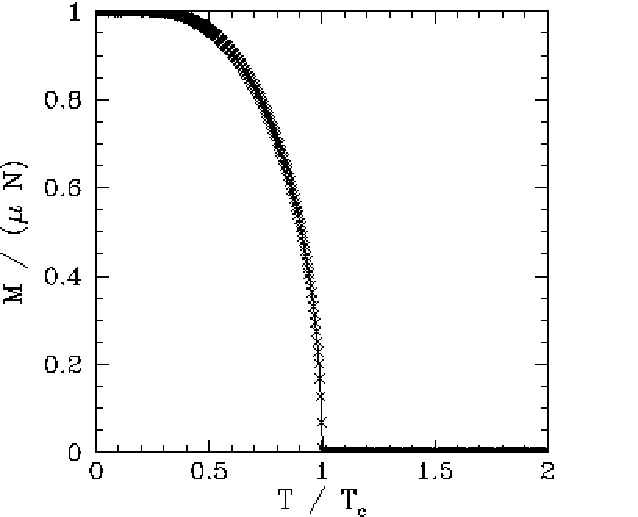
\includegraphics[width=0.98\textwidth]{magTherm}
\end{subfigure}
\begin{subfigure}[b]{0.33\textwidth} 
  \centering
    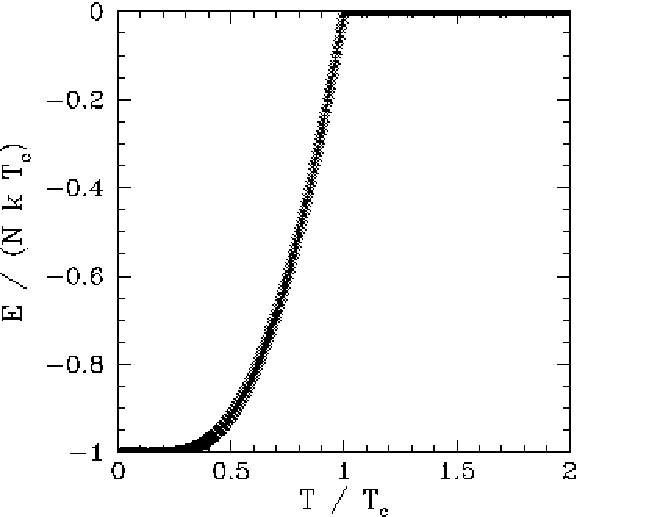
\includegraphics[width=\textwidth]{eTherm}
\end{subfigure}
\begin{subfigure}[b]{0.33\textwidth} 
  \centering
    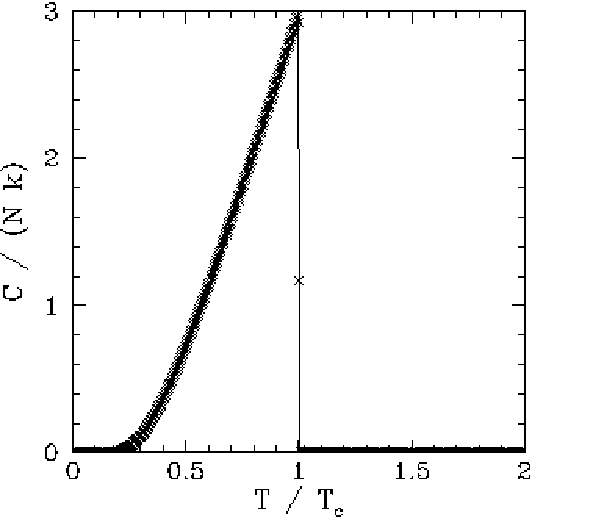
\includegraphics[width=0.93\textwidth]{cTherm}
\end{subfigure}
\caption{The magnetisation per spin $M$, energy per spin $E$ and the specific heat per spin $c$ as calculated in the thermodynamic ($N \to \infty$) limit. Calculated using the mean-field method. At $T_C$ the discontinuity that gives rise to the phase transition is visible. Source: \cite{therm}. }
  \label{fig:obstherm}
\end{figure}

These observables have a discontinuity at a finite temperature, this is the critical temperature where the zero field Ising model has a phase transition. The temperature at which this phase transition occurs is called $T_C$ and can by analytically found to be equal to $k_B T_C / J = \frac{2}{\ln(1 + \sqrt{2})} \simeq 2.2691 \dots $ (see for example Onsager 1944 \cite{onsager} for a derivation). We often define a reduced temperature $\tilde{T} = k_B T / J$ for notational clarity where the tilde is often dropped. We will adopt this practice in the rest of the report. In this convention the critical temperature is denoted as $T_C = \frac{2}{\ln(1 + \sqrt{2})} \simeq 2.2691 \dots$.

\subsection{Restricted Boltzmann Machines}

Restricted Boltzmann Machines (RBM) are a class of neural networks that consist of a hidden and a visible layer where the only connections are between the two layers (no connections between 2 visible or 2 hidden nodes, see figure \ref{fig:RBM}). In a RBM the nodes can have values in $\{0,1\}$.

\begin{figure}[H] 
\centering
\todo[inline]{Removed sourced image.}
\caption{General structure of the Restricted Boltzmann Machine with visible nodes $v$ and hidden nodes $h$ with a bias $a$ and $b$ for the visible and the hidden layer respectively. The connections between the visible and the hidden layer are given by the weight matrix $W$. Note that there are no connections between nodes within each of the layers. Source: \cite{RBM}. }
\label{fig:RBM}
\end{figure}

\newpage

A RBM can be used as a model of a probability density function $P$ where $P$ is defined as

\begin{align}
P(\mathbf{v},\mathbf{h}) = \frac{e^{-E(\mathbf{v},\mathbf{h})}}{Z}
\end{align}

where $\mathbf{v}$ and $\mathbf{h}$ denote the visible and the hidden layer respectively, $E$ is defined by

\begin{align*}
E(\mathbf{v},\mathbf{h}) = -\mathbf{a}^{\mathrm{T}} \mathbf{v} -\mathbf{b}^{\mathrm{T}} \mathbf{b} - -\mathbf{v}^{\mathrm{T}} W \mathbf{h}
\end{align*}

where $\mathbf{a}$ and $\mathbf{b}$ are the biases of the visible and the hidden layers respectively and $W$ is the weight matrix.
\\
\\
The normalisation factor $Z$ (often called the partition function analogously with the partition function found in statistical mechanics) is defined by

\begin{align*}
Z = \sum_{\mathbf{v},\mathbf{h}} E(\mathbf{v},\mathbf{h})
\end{align*}

where the sum goes over all the possible configurations of $\mathbf{v}$ and $\mathbf{h}$.
\\
\\
$P$ is modelled by feeding the RBM a set of inputs and maximizing the log likelihood by using a technique called contrastive divergence. Once $P$ is modelled the RBM can be used to generate new samples from this this distribution using Gibbs sampling (figure \ref{fig:GibbSample}). See for example Salakhutdinov et al. 2007 \cite{RBMpaper} for a detailed explanation.

\begin{figure}[H] 
\centering
\todo[inline]{Removed sourced image.}
\caption{Gibbs sampling used to generate new data points corresponding the the probability distribution of the trained Restricted Boltzmann Machine. Source: \cite{RBM}.}
\label{fig:GibbSample}
\end{figure}


\section{Methods} \label{sec:methods}

\subsection{Data generation (MCMC)}

In order to approximate the observables defined in section \ref{sec:ising} we first need to train the RBM. In order to do this a collection of lattices with $N$ spins were generated using the conventional MCMC method. Lattices were generated in a range of temperatures $T$ with a step size $\Delta T$, at each temperature we generate $n$ independent lattices and use those lattices to train the Restricted Boltzmann Machines, one RBM for each temperature in the range. The values of $T$, $\Delta T$ and $n$ used are given in table \ref{tab:MCMCparam}. The resulting dataset consists of 7500 lattices which were used to train 40 independent RBMs and this dataset is visualized in figure \ref{fig:dataset}. The dataset behaves as expected with all spins aligned in the low temperature region and random spins in the high temperature region.

\begin{table}[H] 
\centering
\caption{Parameters used to generate the data set used to train the RBMs.}
\begin{tabular}{l|ll}
Parameter: & Value: &  \\ 
\hline \hline
$T_\mathrm{min}$     & $1.0$                    \\
$T_\mathrm{max}$     & $4.0$                        \\
$\Delta T$    & $0.1$                        \\
$N$     & $16 \times 16$                       \\
$n$     & $250$                         \\  
\end{tabular}
\label{tab:MCMCparam}
\end{table}

\begin{figure}[H] 
\begin{subfigure}[b]{0.5\textwidth}
  \centering
    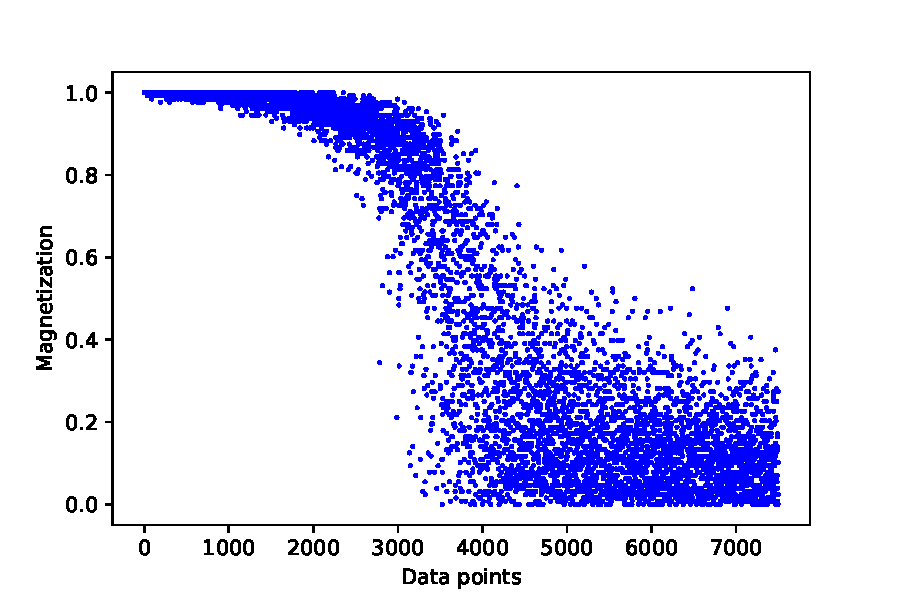
\includegraphics[width=\textwidth]{mag}
    \subcaption{}
\end{subfigure}
\begin{subfigure}[b]{0.5\textwidth} 
  \centering
    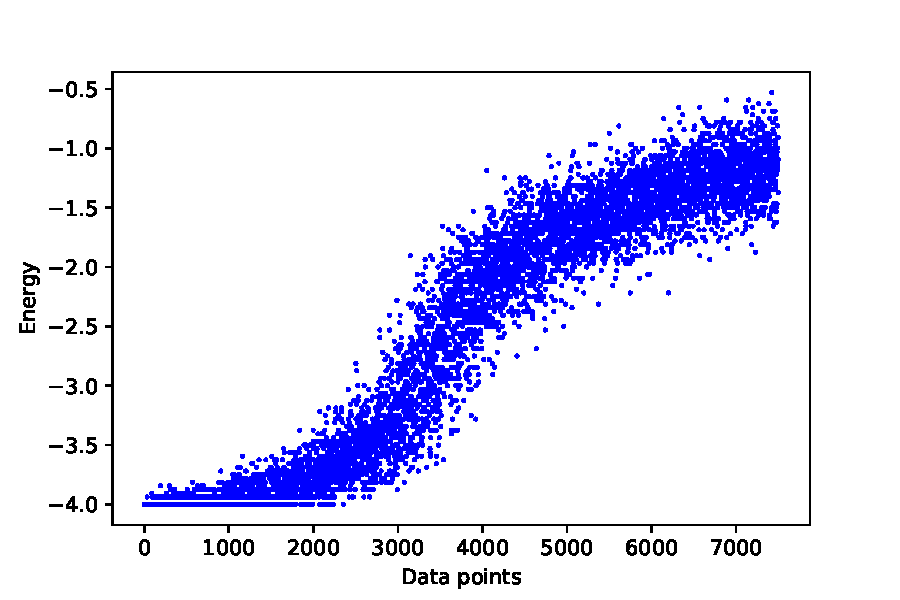
\includegraphics[width=\textwidth]{energy}
    \subcaption{}
\end{subfigure}
\caption{Visualization of the dataset that was generated to train the RBMs. Generated using MCMC with the parameters as given in table \ref{tab:MCMCparam}. Figure a and b respectively show the magnetisation per spin and energy per spin for each lattice in the dataset. The data points are ordered in increasing temperature.}
  \label{fig:dataset}
\end{figure}

\subsection{Restricted Boltzmann Machines}

In order to train the RBMs we convert each of the lattices to vectors of length $N$ and we change the values from {-1,+1} to {0,1} in order to make them compatible with the RBM structure. Each spin in the lattice is represented by 1 visible node in the RBM.
\\
\\
The main parameter we want to look at is the number of hidden nodes $N_h$ in the network. The number of visible nodes $N_v$ is defined by the number of spins in the lattice. The number of hidden nodes $N_h$ can be varied. 
\\
\\
The other parameters of the RBM are the learning rate, the number of iterations and the batch size. In order to tune these parameters we looked at a single temperature dataset at a temperature at approximately the critical temperature. This temperature is chosen because it is expected that the RBM will take the longest time to reach max likelihood around this phase transition. We run the model with varying values for the parameters and look with which values the best likelihood is achieved. After the process the parameters were chosen as given in table 

\begin{table}[H] 
\centering
\caption{Parameters used to train the Restricted Boltzmann Machines.}
\begin{tabular}{l|ll}
Parameter: & Value: &  \\ 
\hline \hline
batch size     & $10$                    \\
$N_\mathrm{itr}$     & $100$                        \\
Learn rate    & $0.001$                        \\  
\end{tabular}
\label{tab:rbmpar}
\end{table}

After training we use the trained models to generate new data using Gibbs sampling at each temperature. After equilibration these generated lattices are sampled and from these sample the observables are calculated using the definitions given in section \ref{sec:ising}.

\subsection{Implementation}

The RBM was implemented using the Bernoulli Restricted Boltzmann Machine from scikit learn 0.20.3. The plots were made using Matplotlib 3.0.3. Both were implemented using Python 3.6.8.

\newpage

\section{Results}

The first results we look at is the three observables calculated with 256 hidden nodes, so there are a equal amount of hidden and visible nodes in the network. In figure \ref{fig:magRBM1} we can see that the magnetisation per spin generated using the RBM has the same shape as the thermodynamic result shown in figure \ref{fig:magRBM1}. As expected the magnetisation tends to $\pm 1$ at low temperatures and tends to zero at high temperatures. It also has a discontinuity around $T_C$.

\begin{figure}[H] 
\centering
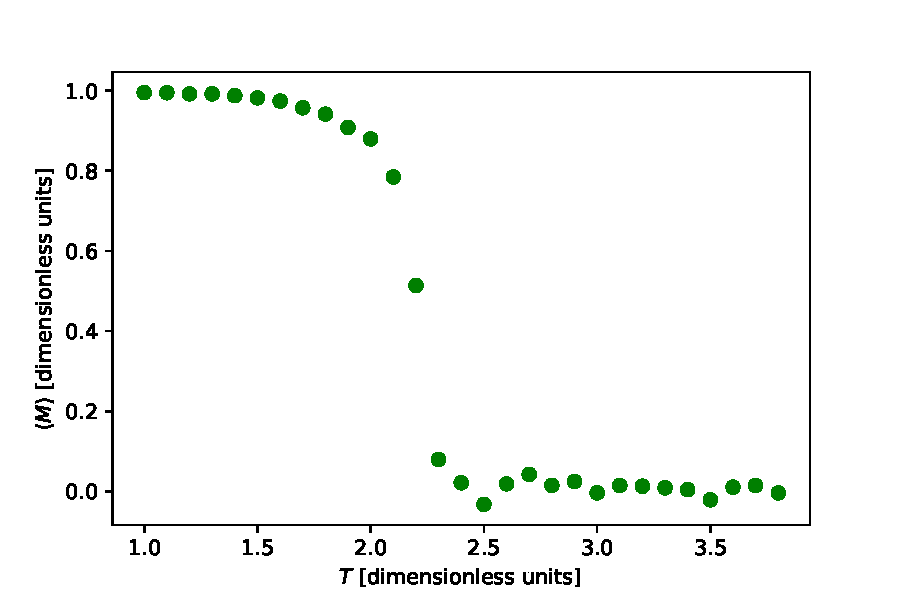
\includegraphics[width=0.7\textwidth]{magRBM}
\caption{The magnetisation per spin $M$ as calculated using the trained RBM with $N_h = 256$ and the other parameters as given in table \ref{tab:rbmpar}. The magnetisation per spin goes to $+1$ at low temperatures and to 0 at high temperatures and has a discontinuity around $T_C$.}
\label{fig:magRBM1}
\end{figure}

In figure \ref{fig:eRBM1} we see that the energy per spin agrees with the analytical results in thermodynamic limit as well. It goes to $-4$ in the low temperature limit which agrees with the expectation that all spins are aligned in the low temperature region and $J > 0$. For high temperatures it goes to 0 which is consistent with all spins being random. Around $T_C$ is has a discontinuity.

\begin{figure}[H] 
\centering
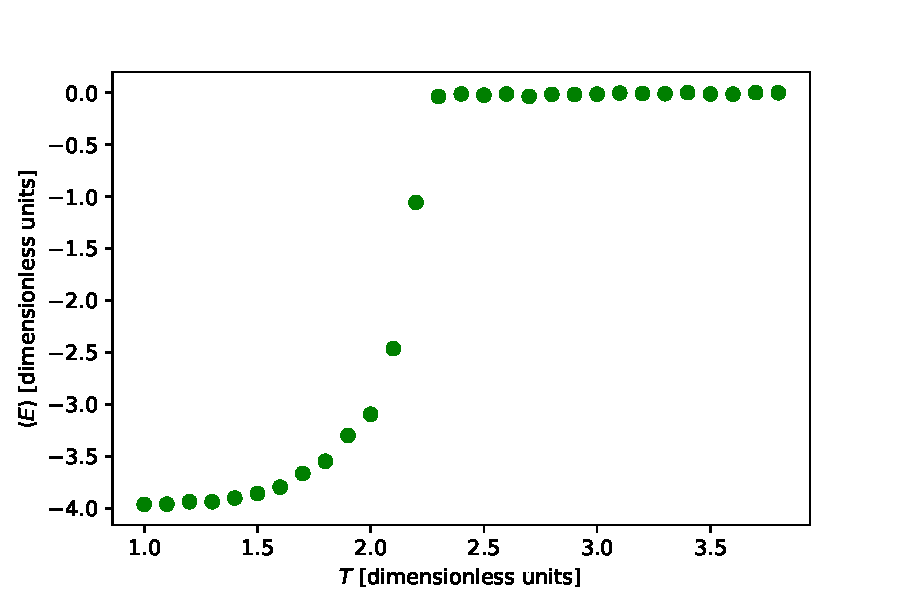
\includegraphics[width=0.7\textwidth]{eRBM}
\caption{The energy per spin $E$ as calculated using the trained RBM with $N_h = 256$ and the other parameters as given in table \ref{tab:rbmpar}. The energy per spin goes to $-4$ at low temperatures and to 0 at high temperatures and has a discontinuity around $T_C$. }
\label{fig:eRBM1}
\end{figure}

In figure \ref{fig:cRBM1} we see that the specific heat per spin as calculated using the RBM has the same shape around the phase transition as the analytical results with a discontinuity around $T_C$. Above and below this temperature the specific heat per spin does not go to zero which is different then the analytical results. For the specific heat per spin to go to zero the variance of the energy should go to zero which is difficult in a random simulation such as using a RBM. Simulating the specific heat per spin using MCMC gives the same difference between computational result and analytical result.

\begin{figure}[H] 
\centering
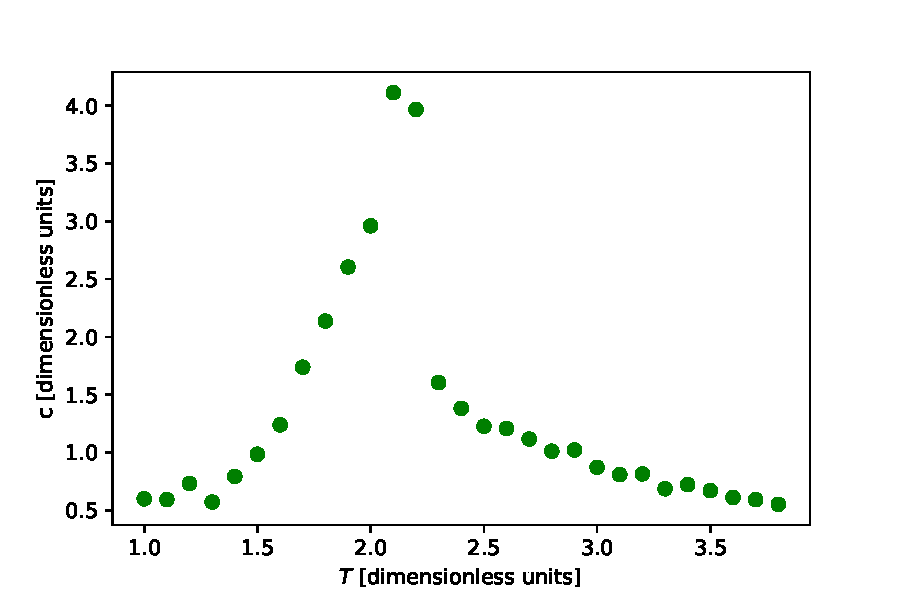
\includegraphics[width=0.7\textwidth]{cRBM}
\caption{The specific heat per spin $c$ as calculated using the trained RBM with $\alpha = 1$ and the other parameters as given in table \ref{tab:rbmpar}.}
\label{fig:cRBM1}
\end{figure}

When we vary the number of hidden nodes we see that the magnetisation per spin (figure \ref{fig:magRBMmul}) still goes to zero in the high temperature region and still has a discontinuity around $T_C$. However in the low temperature region we see that the magnetisation per spin equilibrates to a value $< +1$. This is the same effect as applying an external magnetic field to the Ising model would have. Introducing an external magnetic field reduces the dominance of the coupling constant $J$ on the system so it has the effect of reducing the strength of the coupling. Reducing the number of hidden nodes also has the potential effect of reducing the coupling strength between visible nodes which might be an explanation for the observed equilibration to a value $< +1$.

\begin{figure}[H] 
\centering
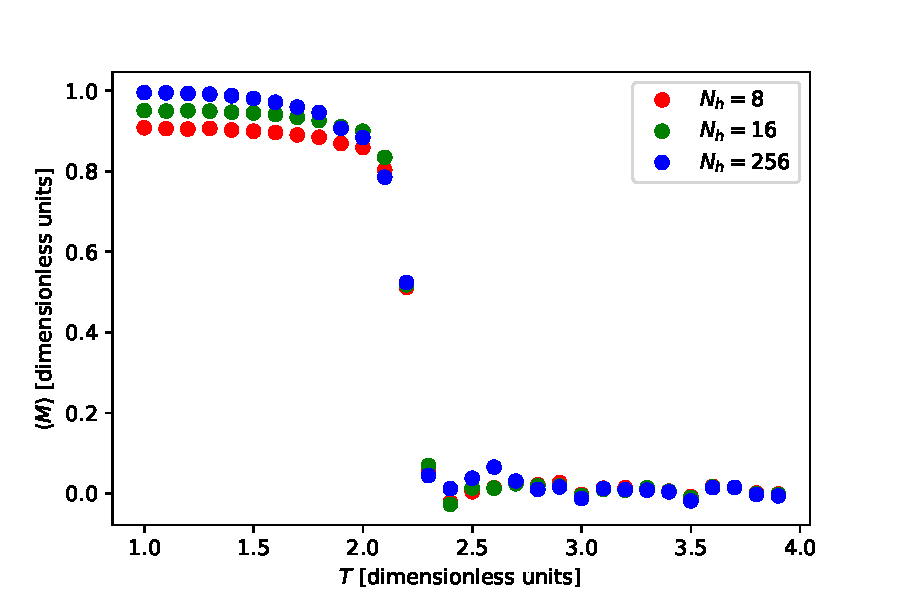
\includegraphics[width=0.7\textwidth]{magRBMmulti}
\caption{The magnetisation per spin $M$ as calculated using the trained RBM with $N_h$ as given in the legend and the other parameters as given in table \ref{tab:rbmpar}. For all values of $N_h$ the system has the discontinuity. In the low temperature region a difference can be seen between the values of $N_h$. }
\label{fig:magRBMmul}
\end{figure}

For the energy per spin (figure \ref{fig:eRBMmul}) we observe a similar effect. It still goes to zero in the high temperature region and has a discontinuity around $T_C$. In the low temperature region it equilibrates to a value $> -4$ which is the same effect as lowering the value of the coupling constant $J$. So for the energy per spin we also observe that lowering the number of hidden nodes gives the same effect as reducing the (relative) coupling strength between the spins.

\begin{figure}[H] 
\centering
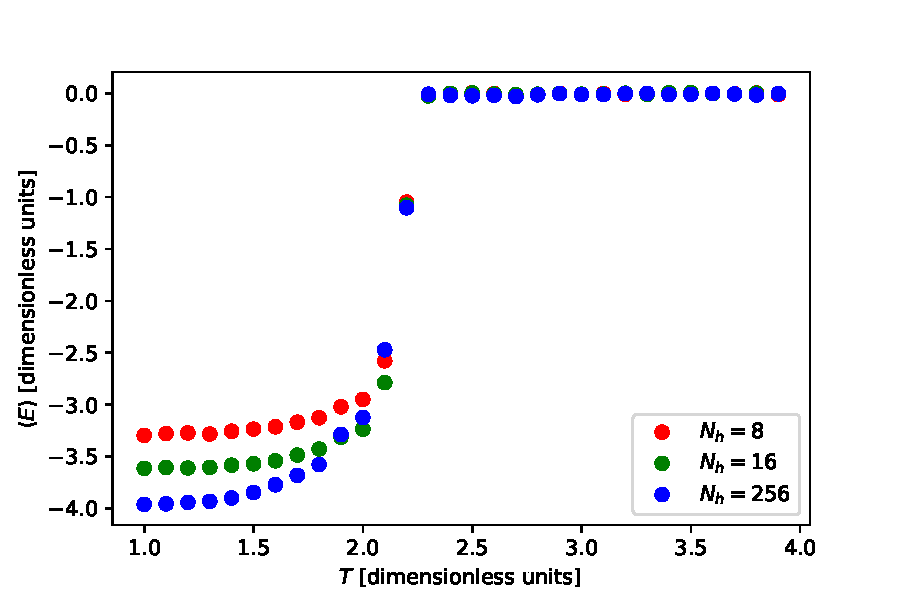
\includegraphics[width=0.7\textwidth]{eRBMmulti}
\caption{The energy per spin $E$ as calculated using the trained RBM with $N_h$ as given in the legend and the other parameters as given in table \ref{tab:rbmpar}. For all values of $N_h$ the system has the discontinuity. In the low temperature region a difference can be seen between the values of $N_h$. }
\label{fig:eRBMmul}
\end{figure}

\newpage

For the specific heat per spin (figure \ref{fig:cRBMmul}) we observe that the RBM fails to correctly model the spefic heat per spin when the number of hidden nodes is lowered.

\begin{figure}[H] 
\centering
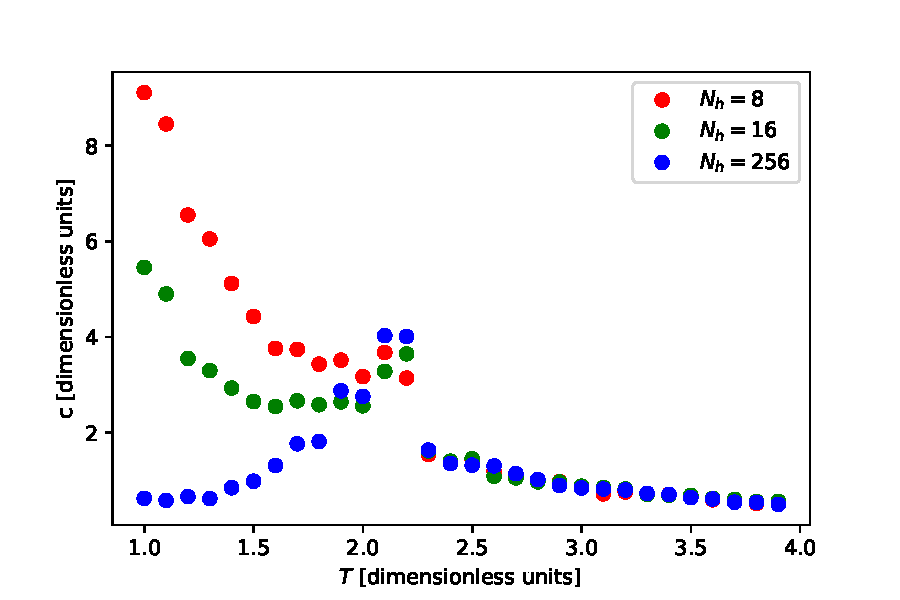
\includegraphics[width=0.7\textwidth]{cRBMmulti}
\caption{The specific heat per spin $c$ as calculated using the trained RBM with $N_h$ as given in the legend and the other parameters as given in table \ref{tab:rbmpar}. For all values of $N_h$ the system has the discontinuity. In the low temperature region a difference can be seen between the values of $N_h$. The system fails to correctly show the behaviour of $c$ in the low temperature region for a low value of $N_h$. }
\label{fig:cRBMmul}
\end{figure}

When we look at the weight matrices for each of the RBMs we see that for the RBM trained at $T = 2.3$ (figure \ref{fig:weightcrit}) we see the structure commonly found when looking at the probability measure of the Ising model. 

\begin{figure}[H]
  \centering
    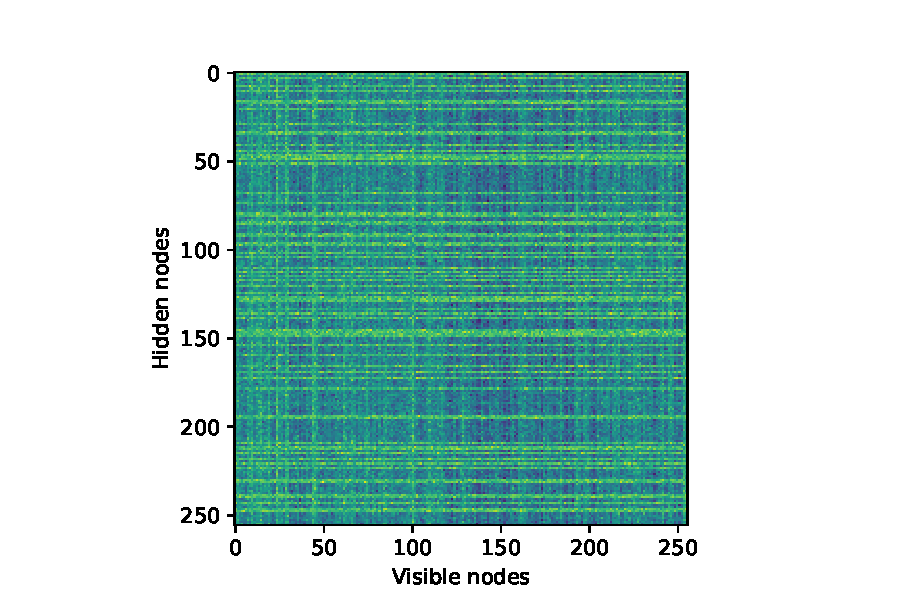
\includegraphics[width=0.6\textwidth]{weightsCrit}
    \caption{The weight matrix for a RBM with $N_h = 256$ trained on the Ising model data at approximately the critical temperature ($T = 2.3$). One can see the structure and order at different length scales which give rise to the interaction between visible nodes and resembles the probility measures often found in the study of the Ising model. \label{fig:weightcrit}}
\end{figure}

\newpage

However when we look at the weight matrix below ($T = 1$) and above ($T = 3.9$) in figure \ref{fig:weightlowhigh} we see that they look equal and random which is surprising since the model behaves quite differently in these two temperature regions.

\begin{figure}[H] 
\begin{subfigure}[b]{0.5\textwidth}
  \centering
    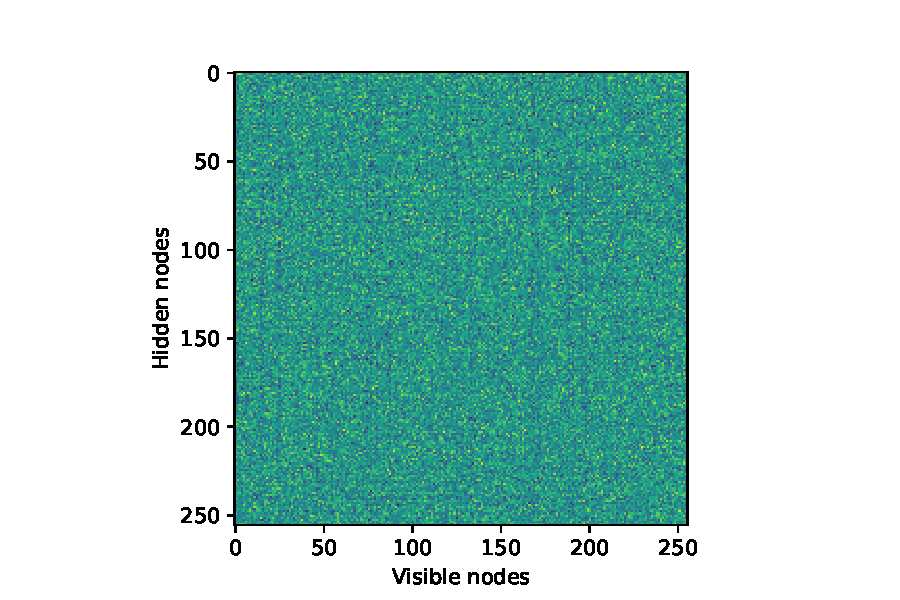
\includegraphics[width=\textwidth]{weightsLow}
    \subcaption{$T = 1.0$}
\end{subfigure}
\begin{subfigure}[b]{0.5\textwidth} 
  \centering
    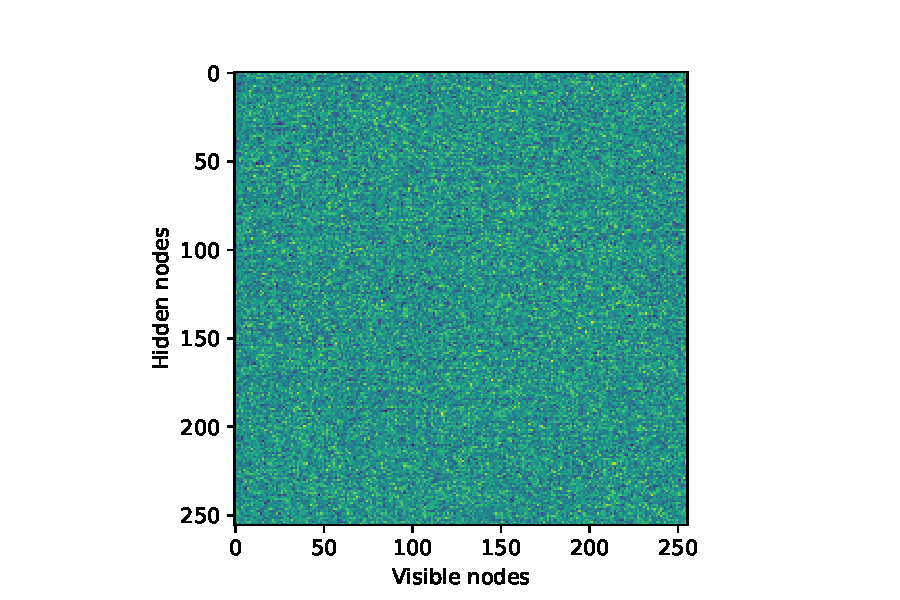
\includegraphics[width=\textwidth]{weightsHigh}
    \subcaption{$T = 3.9$}
\end{subfigure}
\caption{The weight matrix for a RBM with $N_h = 256$ trained on the Ising model data at below and above the critical temperature (see subcaption for temperatures). There is no apparent structure in both of these temperature ranges, this in contrast to the weight matrix around the critical temperature (figure \ref{fig:weightcrit}). Both these matrix look equal and random.}
  \label{fig:weightlowhigh}
\end{figure}

\section{Conclusion}

We found that RBMs for $N_h = N_v$ manage to generate lattices that can be used to calculate the magnetisation per spin, energy per spin and specific heat per spin such that they agree with physical intuition and with the analytical results found using mean-field methods.
\\
\\
When lookig at lower values of $N_h$ we found that the magnetisation per spin behaves as if there was an external magnetic field. Which is interesting since the RBMs were trained using data generated using a simulation of the zero-field model. The energy per spin shows the same effect for lower values of $N_h$ which behaves the same as for the Ising model with a coupling constant smaller then one.
\\
\\
Both these observations show that when the number of hidden nodes is lowered the system behaves as an Ising model where the relative coupling strength between the spins is lower than that the RBMs were trained at. 
\\
\\
When we compare the RBM results in figures \ref{fig:magRBM1}, \ref{fig:eRBM1} and \ref{fig:cRBM1} with the results from the conventional Markov Chain Monte Carlo we see that the results from the RBM more closely resemble the analytical results than that of the MCMC (figure \ref{fig:obsmcmc}). The analytical results are calculated using the mean-field approximation in which more contributions are taken into account then just the nearest neighbour connections. In the results calculated using MCMC only the nearest neighbour interactions are taken into account. However in the RBM each visible node is connected to more visible nodes (via the hidden nodes) then just the nearest neighbours which might be an explanation why the RBM results more closely resemble the mean-field results than the MCMC results. An interesting remark is that the RBMs used are trained using data that was generated using only nearest neighbour interactions. 

\begin{figure}[H] 
\begin{subfigure}[b]{0.33\textwidth}
  \centering
    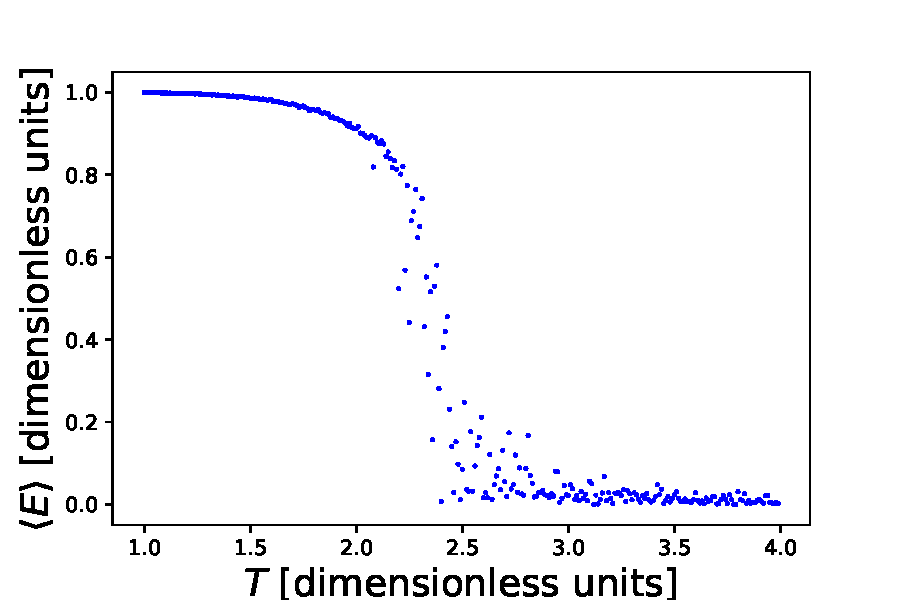
\includegraphics[width=\textwidth]{mMCMC}
\end{subfigure}
\begin{subfigure}[b]{0.33\textwidth} 
  \centering
    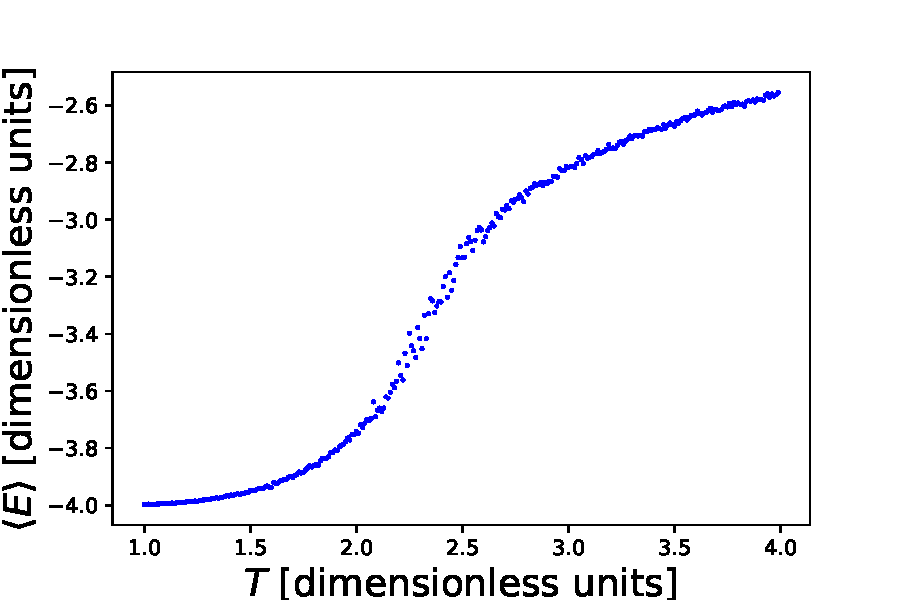
\includegraphics[width=\textwidth]{eMCMC}
\end{subfigure}
\begin{subfigure}[b]{0.33\textwidth} 
  \centering
    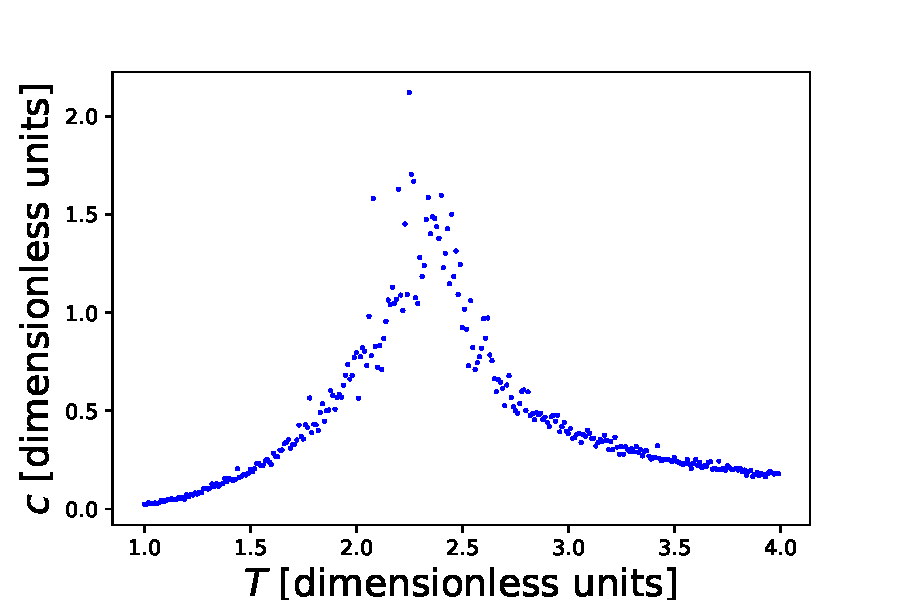
\includegraphics[width=\textwidth]{cMCMC}
\end{subfigure}
\caption{The magnetisation per spin $M$, energy per spin $E$ and the specific heat per spin $c$ as calculated using the MCMC method at a lattice size of $16 \times 16$ where only nearest neighbour contributions to the energy were used. These results resemble the analytical results less closely than the results of the RBMs.}
  \label{fig:obsmcmc}
\end{figure}

\begin{thebibliography}{99}
\bibitem{thijssen} 
J.M. Thijssen (2013), \textit{Computational Physics}, Cambridge University Press, Cambridge, UK.

\bibitem{therm}
Richard Fitzpatrick - The Ising Model, \url{http://farside.ph.utexas.edu/teaching/329/lectures/node110.html}, Retrieved on 21-5-2019.

\bibitem{onsager}
L. Onsager (1944), \textit{"Crystal statistics. I. A two-dimensional model with an order-disorder transition"}, Physical Review, Series II, 65 (3–4): 117–149.

\bibitem{RBM}
Towards Data Science - Deep Learning meets Physics: Restricted Boltzmann Machines \url{https://towardsdatascience.com/deep-learning-meets-physics-restricted-boltzmann-machines-part-i-6df5c4918c15}, Retrieved on 20-5-2019.

\bibitem{RBMpaper}
Salakhutdinov et al. (2007), \textit{Restricted Boltzmann Machines
for Collaborative Filtering}, ICML '07, pg. 791-798.

\bibitem{scikit}
SciKit Learn documentation - Bernoulli Restricted Botlzmann Machine, \url{https://scikit-learn.org/stable/modules/generated/sklearn.neural_network.BernoulliRBM.html}, Retrieved on 19-5-2019.

\end{thebibliography}
\end{document}